\documentclass[acmtog]{acmart}
\usepackage{graphicx}
\usepackage{subfigure}
\usepackage{natbib}
\usepackage{listings}
\usepackage{bm}
\usepackage{amsmath}

\definecolor{blve}{rgb}{0.3372549 , 0.61176471, 0.83921569}
\definecolor{gr33n}{rgb}{0.29019608, 0.7372549, 0.64705882}
\makeatletter
\lst@InstallKeywords k{class}{classstyle}\slshape{classstyle}{}ld
\makeatother
\lstset{language=C++,
	basicstyle=\ttfamily,
	keywordstyle=\color{blve}\ttfamily,
	stringstyle=\color{red}\ttfamily,
	commentstyle=\color{magenta}\ttfamily,
	morecomment=[l][\color{magenta}]{\#},
	classstyle = \bfseries\color{gr33n}, 
	tabsize=2
}
\lstset{basicstyle=\ttfamily}

% Title portion
\title{Assignment 3: {Ray Tracing Basics}} 

\author{Name:\quad Yin Hairui  \\ student number:\ 2020533028
\\email:\quad yinhr@shanghaitech.edu.cn}

% Document starts
\begin{document}
\maketitle

\vspace*{2 ex}

\section{Introduction}
In this assignment, we are asked to render a scene by simple ray tracing with area light. Camera generates rays to pixel on the screen plane and ray sintersect with objects. After calculation, we can get the radiance of the pixel which contributes to the whole photo.\\ The followings are all jobs that have been doen, containing basic task and texture!
\begin{itemize}
	\item generate rays from camera
	\item ray geometry intersection
	\item Phong lighting at intersection
	\item light ray sampling for soft shadow
	\item anti-aliasing by super-resolution
	\item texture mapping
\end{itemize}
\section{Implementation Details}
\subsection{Camera Rays}
There are elements that we are required to define in camera class:
\begin{itemize}
	\item Forward: a normalized vector pointing at where the camera looks at
	\item Right: a normalized vector pointing at the right side of camera
	\item Up: a normalized vector pointing at the up side of camera
\end{itemize}
To generate a ray from the camera, two floating number 'dx' and 'dy' are given, specifying the ray’s location on raster space. Then we need to calculate the coordinate in world space of this point.\\
The 'dx' and 'dy' has range of $$dx\in [0, resolution.x()),dy\in [0, resolution.y())$$ which give a percentage position of the current raster. To ease the calculation of ray sample, I return the lower left corner of grids that divides the raster.\\
$$LC=SC-H_n * s_x / 2 - V_n * s_y / 2$$
Where $LC$ is lower left corner, $SC$ is the screen center, $H_n$ is the normalized vertor in horizon, $s_x$ is the size of resolution in horizon direction, $V_n$ is the normalized vertor in vertical, $s_y$ is the size of resolution in vertical direction.
\subsection{Geometry Intersection}
Given a ray, the geometry intersection part gives the answer of whether the ray intersects with any geometry and returns a element called 'interaction' recording all imformation about the intersection, containing
\begin{itemize}
	\item type: Can be "NONE", "GEOMETRY" or "LIGHT", meaning what the ray first intersects
	\item pos: the position where intersection happens
	\item dist: the distance between ray.origin and intersection position
	\item normal: normal vector of the intersection point
	\item uv: a percentage variable giving ways for texture mapping
	\item model: phone light model telling the properties of light in this intersecting position
\end{itemize}
There are three types of geometries we define:
\subsubsection{Triangle}
Trianle intersection depends on linear equation
$$o+td=(1-b_1-b_2)P_0+b_1P_1+b_2P_2$$
\subsubsection{Rectangle}
Rectangle has a similar formula as triangle and a little adjustment in the range of $b_1,b_2$.
\subsubsection{Ellipsoid}
Ellipsoid is a little bit difficult. Since we can transform a sphere to ellipsoid with scaling, rotating and transforming, the transmitting matrix can be generated. We use the inverse of the matrix to do transformation in our ray and find out the intersection of transformed ray and unit sphere. After finding the intersection, we use $t$ in the transformed ray equation in untransformed one, which gives us the intersection of ray and ellipsoid. And normal has a more difficult calculating method.
$$Normal = M_inverse.eval().transpose() \times Sphere_n$$
\subsection{Phone lighting}
Given a light with color, phone lighting represents how the object interacts with the light. It has three components: Ambient, Diffuse and Specular. We load these components when intersect with geometries.
\subsubsection{Ambient Light: }
Ambient light comes from the refleciton of surrounding environment. There is a constant defining the strength of ambient light.
\subsubsection{Diffuse Light: }
Diffuse light is determined by the angle between light and normal of that position. After normalizing these two vectors, I use dot product to find the cos(angle) and mutiple it with light to calculate diffuse light. Bigger the angle is, Weaker is the diffuse light.
\subsubsection{Specular Light: }
As light hit a surface, there is a reflect angle. If we are in the angle of outgoing light, the object will seem glossy. Specular Light calculates the angle between our view direction and the reflecting direction. It has the same calculating order as diffuse light, first normalizing then dot product.\\
These three light factor interacting with given sampled light altogether are added together distributing to the color in pixels. The calculating procedure in in radiance(), "intergrator.cpp".
\subsection{Soft shadow}
For soft shadow, the area light is divided into several points light, each has a equal weight. I sample it into rectangle grids, center of each as a single light. The sampled area light gives color to pixel where it happend to be blocked by the marginal of geometries in case the pixel becoming full black.
\subsection{Super Resolution}
Similar to Soft shadow, super resolution samples the pixel into many small pixels, each with a weight. Color of the original pixel is generated by the average of each small pixel. However, super resolution treats every pixel equally, which gives too much unnecessary sampling.
\subsection{Texture Mapping}
With lib "stb\_image", we can load images like jpg, png into readable raw data. Texture divides a geometies into different part, and each part has its unique light model. I define a getPixel() function where we can use "u,v"(defined in the part of geometries intersection), to map a texture into geometries according to its percentage.
\section{Results}
The results are pictures following.\\

\begin{figure}[h]
	\centering
	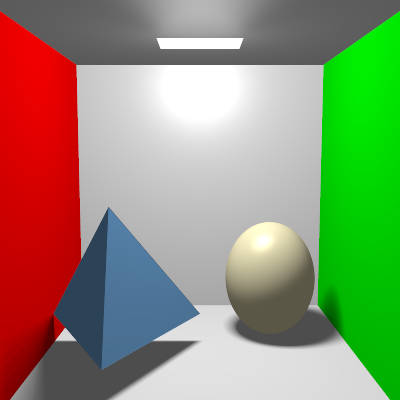
\includegraphics[width=0.7\linewidth]{result_8_5}
	\caption{Origin}
	\label{fig:Origin}
\end{figure}
\begin{figure}[h]
	\centering
	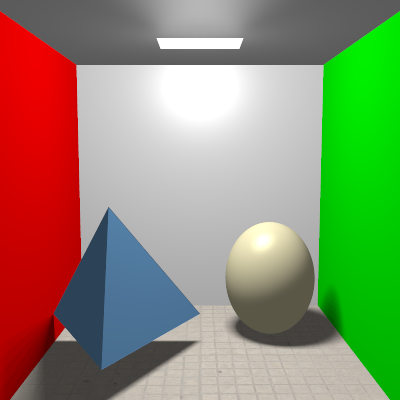
\includegraphics[width=0.7\linewidth]{texture_diff_8_5.png}
	\caption{Render with texture}
	\label{fig:Origin}
\end{figure}
\begin{figure}[h]
	\centering
	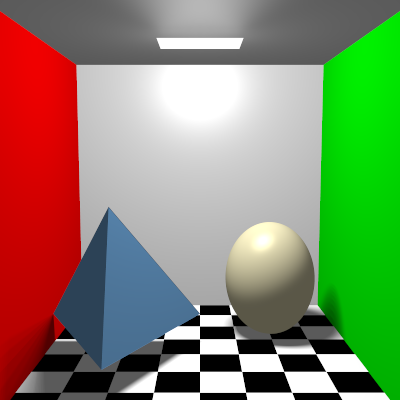
\includegraphics[width=0.7\linewidth]{texture_grid_8_5.png}
	\caption{Render with texture}
	\label{fig:Origin}
\end{figure}

\end{document}
